\documentclass[a5,tombow,multijfont]{ttclass}
\usepackage{makeidx,multicol}
\usepackage[noreplace]{otf}
\usepackage[dvipdfmx]{graphicx,color}
\usepackage{amsmath,amssymb,amsfonts}
\usepackage{bm}
\usepackage{ascmac}
%\usepackage{eucal}
%\usepackage{cancel}
%\usepackage{mathrsfs}
\usepackage{wrapfig}
\usepackage{longtable,multirow}
\usepackage{colortbl}
\usepackage{KbTombowPatch}
\usepackage{xparse}
\usepackage{nccmath}
\usepackage{ulem}
\usepackage{framed}
\usepackage{braket}
\usepackage{subfigmat}
\usepackage{emathMw}
\usepackage{my-emathBk}

\usepackage{toukeigaku}%% 統計学の基本設定
%\usepackage{basic}%%     統計学以外で使う基本設定

\usepackage{auh}

\def\theequation{\arabic{equation}}

\graphicspath{{./fig/}{./samplefig/}}

\includeonly{
./sampletexfiles/maegaki,
./sampletexfiles/toukeisample,
./sampletexfiles/Chap01,
./sampletexfiles/shuffleTEST
}

\begin{document}
\frontmatter

\maegaki{まえがき}
○○○○○○○○○○○○○○○○○○○
○○○○○○○○○○○○○○○○○○○
○○○○○○○○○○○○○○○○○○○
○○○○○○○○○○○○○○○○○○○
○○○○○○○○○○○○○○○○○○○
○○○○○○○○○○○○○○○○○○○
○○○○○○○○○○○○○○○○○○○
○○○○○○○○○○○○○○○○○○○
○○○○○○○○○○○○○○○○○○○
○○○○○○○○○○○○○○○○○○○
○○○○○○○○○○○○○○○○○○○
○○○○○○○○○○○○○○○○○○○
○○○○○○○○○○○○○○○○○○○
○○○○○○○○○○○○○○○○○○○
○○○○○○○○○○○○○○○○○○○
○○○○○○○○○○○○○○○○○○○
○○○○○○○○○○○○○○○○○○○
○○○○○○○○○○○○○○○○○○○
○○○○○○○○○○○○○○○○○○○
○○○○○○○○○○○○○○○○○○○
○○○○○○○○○○○○○○○○○○○
○○○○○○○○○○○○○○○○○○○
○○○○○○○○○○○○○○○○○○○
○○○○○○○○○○○○○○○○○○○
○○○○○○○○○○

\vspace{\baselineskip}
\hfill
\begin{tabular}{l@{}}
20XX年X月\\
○○○大学○○\\
○○○○
\end{tabular}
%まえがき
\tableofcontents
\mainmatter
\begin{問題}{事象と確率} % 質量・長さ・時間(電荷)
サイコロを$4$つ投げたとき,次の確率を求めよ.
\\
(1) 出る目がすべて$1$である確率\\
(2) 出る目がすべて同じである確率\\
(3) ある$2$つのサイコロにおいて出る目が異なる確率\\
(4) どのサイコロも異なる目が出る確率
\end{問題}

\begin{解説}
サイコロを投げるような同様のことを繰り返すことが可能な行為を試行といい,その結果ある目が出るというような事柄を事象という。
特に,事象としてもうこれ以上分けることができない事象を根元事象という。例えば,サイコロの例における「偶数の目が出る」という事象は
「$2$の目が出る」,「$4$の目が出る」,「$6$の目が出る」という事象に分けて考えることができるので根元事象ではないが,
「$3$の目が出る」という事象は$3$の目が出る事象以外の場合に分けて考えられないので,根元事象である。
対象とするすべての根元事象からなる事象の集合を全事象と呼び$U$で表すことにする。
また,事象$A$に対して,事象$A$の場合の数を$n(A)$で表すことにする。全事象$U$に対して,そのすべての根元事象が同様に確からしく起こるとき,
事象$A$の起こる確率$P(A)$は$P(A)=\frac{n(A)}{n(U)}$として定義される。

決して起こらない事象を空事象と呼び,$\emptyset$で表す。定義により,$n(\emptyset)=0$であり,$A=\emptyset$ならば$P(A)=\frac{n(\emptyset)}{n(U)}=0$である。
また,$A=U$ならば$P(A)=\frac{n(U)}{n(U)}=1$である。したがって,一般に確率$P(A)$において$0\leq P(A)\leq 1$が成り立つ。
事象$A$に対して,$A$が起こらないという事象を$A$の余事象といい,$\overline{A}$で表す。定義により,$P(U)=P(A)+P(\overline{A})=1$が成り立つ。

$2$つの事象$A,B$に対して,その和集合と積集合によって定まる事象をそれぞれ和事象,積事象といい,$A\cup B$,$A\cap B$で表す。
$A\cap B=\emptyset$であるとき,$A$と$B$は排反であるという。一般に,$P(A\cup B)=P(A)+P(B)-P(A\cap B)$が成り立ち,$A$と$B$が排反ならば$P(A\cup B)=P(A)+P(B)$が成り立つ。
\end{解説}
\begin{解答}

以下では,対象となる$4$つのサイコロをそれぞれ$a,b,c,d$とおき,これらのサイコロを投げたときに出る目をそれぞれ$f(a),f(b),f(c),f(d)$とおき,出た目の結果を
$(f(a),f(b),f(c),f(d))$で表すことにする。

\VS{1}
\noindent
(1) 出る目がすべて$1$であるという事象を$A$とおくと,事象$A$は$(1,1,1,1)$となる根元事象である。したがって,$n(A)=1$が成り立つ。
一方,この場合の全事象$U$における場合の数$n(U)$は,$(f(a),f(b),f(c),f(d))$で表現できるすべての場合の数$6^4=1296$である。
よって,$P(A)=\frac{1}{1296}$

\noindent
(2) 出る目がすべて同じであるという事象を$B$とおくと,事象$B$の起こり得るパターンは\\
$(1,1,1,1), (2,2,2,2), (3,3,3,3), (4,4,4,4), (5,5,5,5), (6,6,6,6)$の6通り
なので,\linebreak
$n(B)=6$である。全事象$U$における$n(U)$は前問で求めたように$n(U)=1296$なので,$P(B)=\frac{6}{1296}=\frac{1}{216}$

\noindent
(3) ある$2$つのサイコロにおいて出る目が異なるという事象を$C$とおくとき,事象$C$は出る目がすべて同じであるという事象$B$の余事象である。
したがって,前問の結果より,$P(C)=1-P(B)=1-\frac{1}{216}=\frac{215}{216}$ 

\noindent
(4) どのサイコロも異なる目が出るという事象を$D$とおく。場合の数$n(D)$については次のように注意深く求める必要がある。まず,$4$つのサイコロ
を区別することを考えず,出る目のみに着目してどの目も異なるパターンの総数を求めよう。これは$1$から$6$の数字から$4$つの数字を取り出す
組合せの数${}_6 \mathrm{C}_4=\frac{6!}{4!2!}=15$である。一方,どの目も異なる$4$つの数字のひと組に対して,$4$つのサイコロ$a,b,c,d$において
その組の出る目を実現するパターンの総数を考えよう。ここでは,話を分かりやすくするために,一つの具体的な数字の組合せを例えば$1,2,3,4$とおいて
そのパターン数を数え上げてみると,$a,b,c,d$の出る目が$1,2,3,4$であるパターンの総数は$1,2,3,4$を並べ替える順列の数${}_4 \mathrm{P}_4=4!=24$に等しい。
従って,$n(D)=15\times 24=360$が成り立つ。よって,$P(D)=\frac{360}{1296}=\frac{5}{18}$
\end{解答}
       %% 統計学サンプル
\makeatletter
\def\dumyword#1{\@tempcnta=#1\relax
	\loop\ifnum\@tempcnta>\z@\advance\@tempcnta-\@ne
	□\repeat
	}
\makeatother

\chapter{概要}
\begin{abstract}
\dumyword{60}
\end{abstract}



\begin{問題}[標準]{ベイズの定理(Bayes' Theorem)}
\begin{minipage}{.5\linewidth}\textsf{minipageのテスト}\parindent1zw\par
有望と思えるガン発見のある検査法が開発された。大病院のガン患者の $97\%$ がこの検査に陽性反応を示し,ガンでない患者の $5\%$ が同じ陽性反応を示したとしよう。病院の患者の $2\%$ がガンにかかっているとするとき,無作為に選んだある患者がこの検査に陽性反応を示したとして,以下の問いに答えよ。
\end{minipage}
\begin{table}\centering
	\caption{tableのテスト}
	\begin{tabular}{|c|c|c|}
		\hline
		A & B & C\\
		\hline
		A & B & C\\
		\hline
		A & B & C\\
		\hline
	\end{tabular}
\end{table}
\begin{figure}\centering
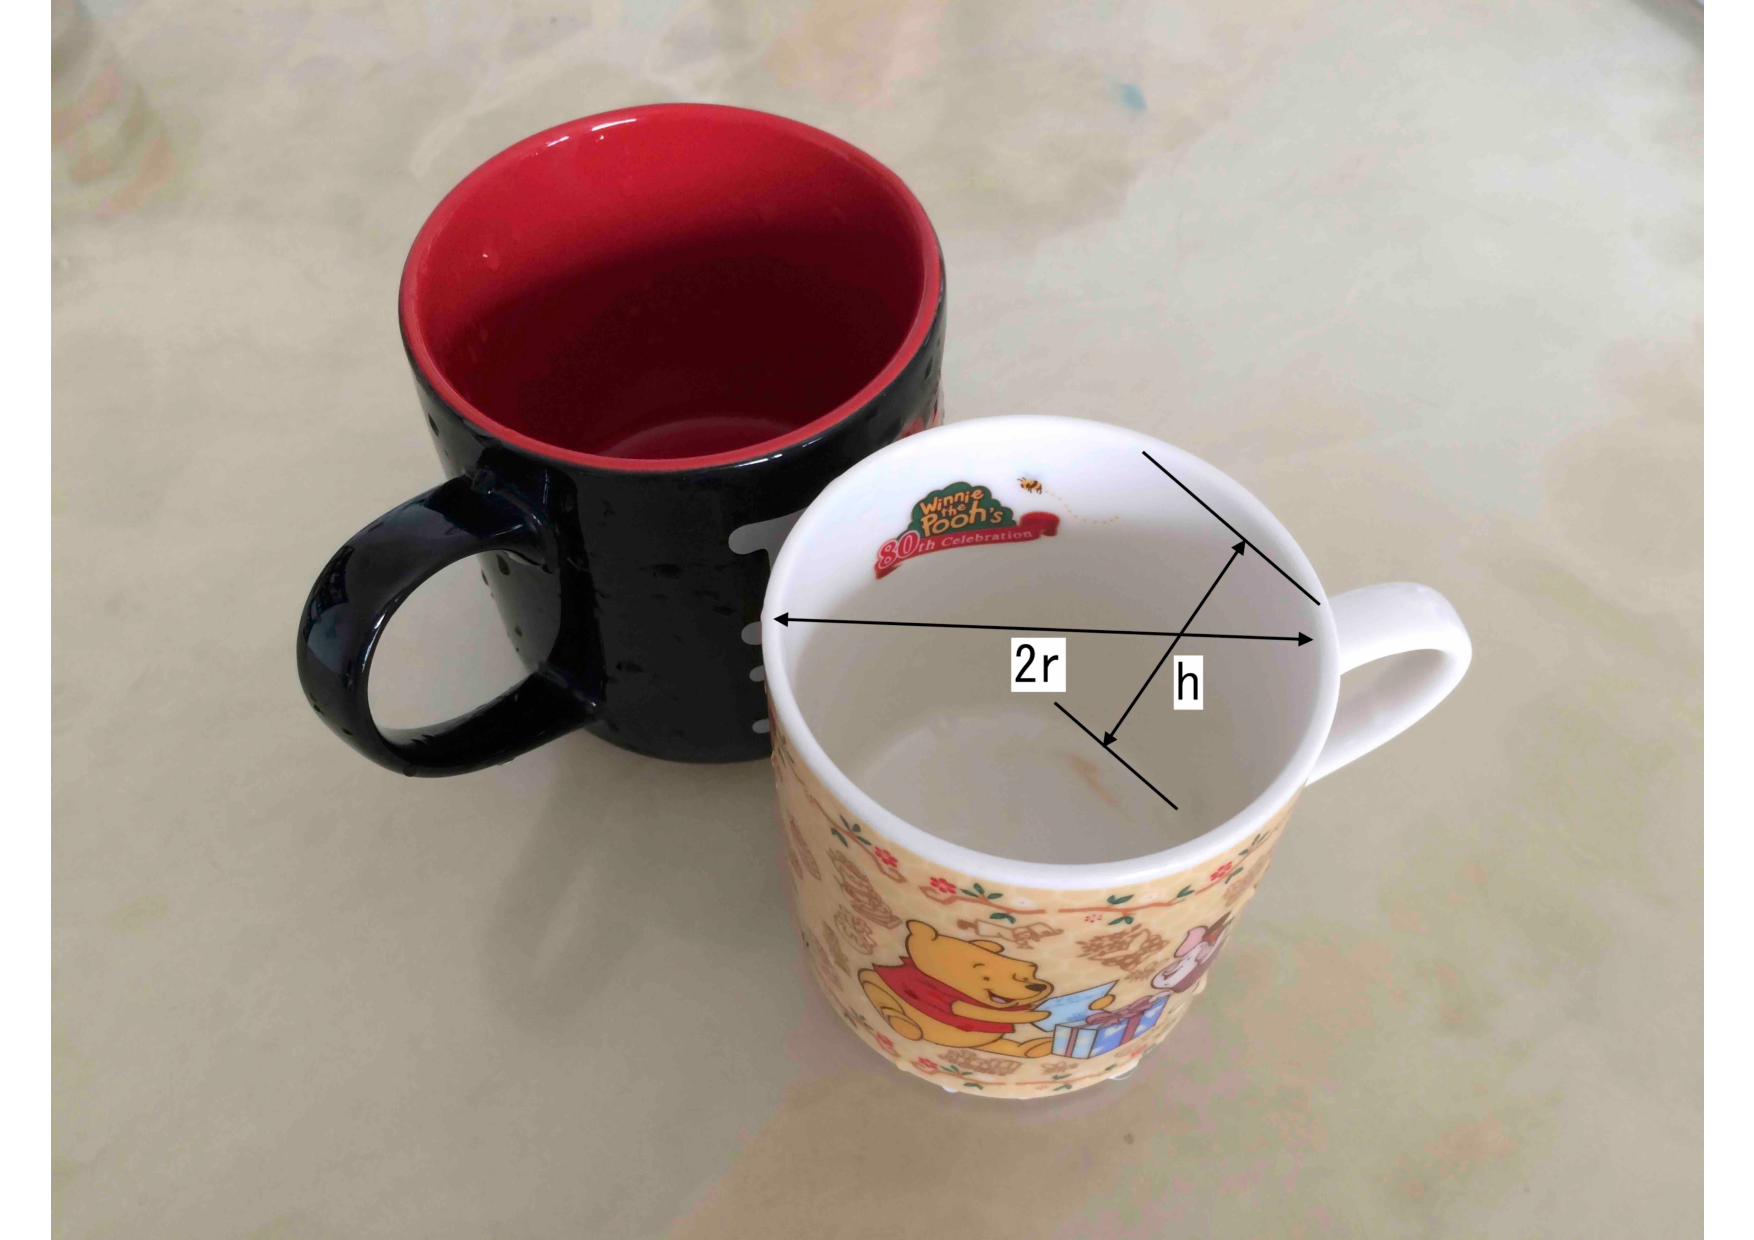
\includegraphics[keepaspectratio,scale=0.17]{cups.pdf}
	\caption{figureのテスト}
\end{figure}

\begin{enumerate}
\item 抽出された患者が本当にガンにかかっている確率を求めよ。
\item (1)で得られた結果について吟味せよ。
\end{enumerate}

\end{問題}

%\dumyword{50}
%\begin{問題}[標準]{TITLE}
%\begin{enumerate}
%\item \dumyword{30}
%\item \dumyword{15}
%\item \dumyword{45}
%\item \dumyword{35}
%\end{enumerate}
%\end{問題}

この問題はベイズの定理(Bayes' Theorem)に対する理解を求めている。

\begin{解説}
まず、ベイズの定理を述べよう。
\begin{網掛け}
$\Omega$ は標本空間で,$H_1,H_2,\cdots, H_k$は$\Omega$の部分集合である。
標本空間 $\Omega$ は$H_1,H_2,\cdots, H_k$によって素分割されている。すなわち、次が成り立つ。
\begin{enumerate}
\item[(1)] $\Omega = H_1\cup H_2\cup\cdots\cup H_k$であり,

\item[(2)] $H_1,H_2,\cdots, H_k$ は互いに排反である。すなわち,$H_i \cap H_j = \phi\, (i\not=j) $である。
\end{enumerate}
このとき,任意の事象$A$と任意$i=1,\cdots, k$に対して,次が成り立つ。
\begin{equation}
P(H_i|A) = 
  {P(H_i)\, P(A|H_i) \over
  \sum_{j=1}^k P(H_j)\, P(A|H_j)}
\label{bayesthm}
\end{equation}
\end{網掛け}
\end{解説}

%\dumyword{40}

%\begin{網掛け}
ベイズの定理は次のように証明される。まず, 事象$A$は$\Omega$の部分集合なので,
集合の吸収則により,$A= A\cap \Omega$となる。条件により,
$
\Omega = H_1\cup H_2\cup\cdots\cup H_k
$
なので,集合の分配則により,
$$
A = (A\cap H_1)\cup (A\cap H_2) \cup\cdots\cup (A\cap H_k)
$$
が成り立つ。確率の加法性により,$A$の確率は
\begin{equation}
P(A) = \sum_{j=1}^k P(A\cap H_j) = \sum_{j=1}^k P(H_j)\, P(A | H_j)
\label{eqn:thmtotal}
\end{equation}
と分解できる。2番目の等号は乗法定理 $P(A\cap B) = P(B)\, P(A | B)$ による。(\ref{eqn:thmtotal})は
{\bf 全確率の定理}(law of total probability)として知られる。条件付確率の定義により,
$$
P(H_i|A) = {P(A\cap H_i) \over P(A)} = {P(H_i)\, P(A|H_i) \over P(A)} 
$$
と書ける。上の式の分母に全確率の定理を適用すれば,ベイズの定理 (\ref{bayesthm})が得られる。

%\end{網掛け}


\begin{解答}
\begin{enumerate}
\item[(1)] 患者の集団を$\Omega$とし,ガン患者の集団を$H_1$, ガンでない患者の集団を$H_2$とすると,$\Omega$は
$H_1$と$H_2$に素分割される。無作為に選んだ患者が陽性を示すという事象を$A$とすると,求めるべき確率は
$P(H_1|A)$と表現できる。以上の記号の下で,与えられた条件は以下のように整理できよう。

\begin{center}
  \begin{tabular}{c|c} \hline
    事前確率 & 尤度 \\ \hline 
    $P(H_1)= 0.02 $ & $ P(A|H_1) = 0.97$ \\
    $P(H_2)= 0.98$ & $P(A|H_2) = 0.05$ \\ \hline
  \end{tabular}
\end{center}

したがって, 全確率は
$$
P(A) =  P(H_1) \, P(A|H_1) + P(H_2) \, P(A|H_2) = 0.02\times 0.97 + 0.98 \times 0.05 = 0.0684
$$
となる。ベイズの定理より
$$
P(H_1|A) = {P(A|H_1) \, P(H_1) \over P(A)} = {0.02\times 0.97 \over 0.0684} \approx 0.284 = 28.4\%
$$

%\footnote{□□□□□□□□□□}

\item[(2)] ベイズの定理における $P(H_i)$は事前確率(prior probability)と呼ばれ,これまでの経験などに基づいて,病気などにおける確率に関する先験的(prior)知識を表す。新たなデータ$A$が得られたとき,病気になる事後確率(posterior probability)$P(H_i|A)$を計算しているのがベイズの定理である。より広い文脈において,$H_i$を原因,$A$を結果とすると,ベイズの定理は,結果が得られたときの原因の確率$P(H_i|A)$を更新するための理論として非常に重要である。

上の例において,$P(H_1|A) = 28.4\%$ がそれほど高くないことに意外と感じるかもしれない。
これがむしろ一般的な現象である。もし,
$\Omega = H_1\cup H_2$ で,$P(H_1)$ が非常に小さければ,$P(H_2) = 1- P(H_1) \approx 1$ となる。
$P(A) \approx P(A|H_2)$となることに注意すれば,
$
P(H_1|A) \approx 0 /  P(A|H_2) = 0
$
となることが理解できよう。
\end{enumerate}

\end{解答}
%\dumyword{60}

\begin{問題}[やや難]{正規分布$N(\mu, 1)$の$2$乗の分布}
\begin{wrapfigure}[9]{l}{50mm} 
\centering
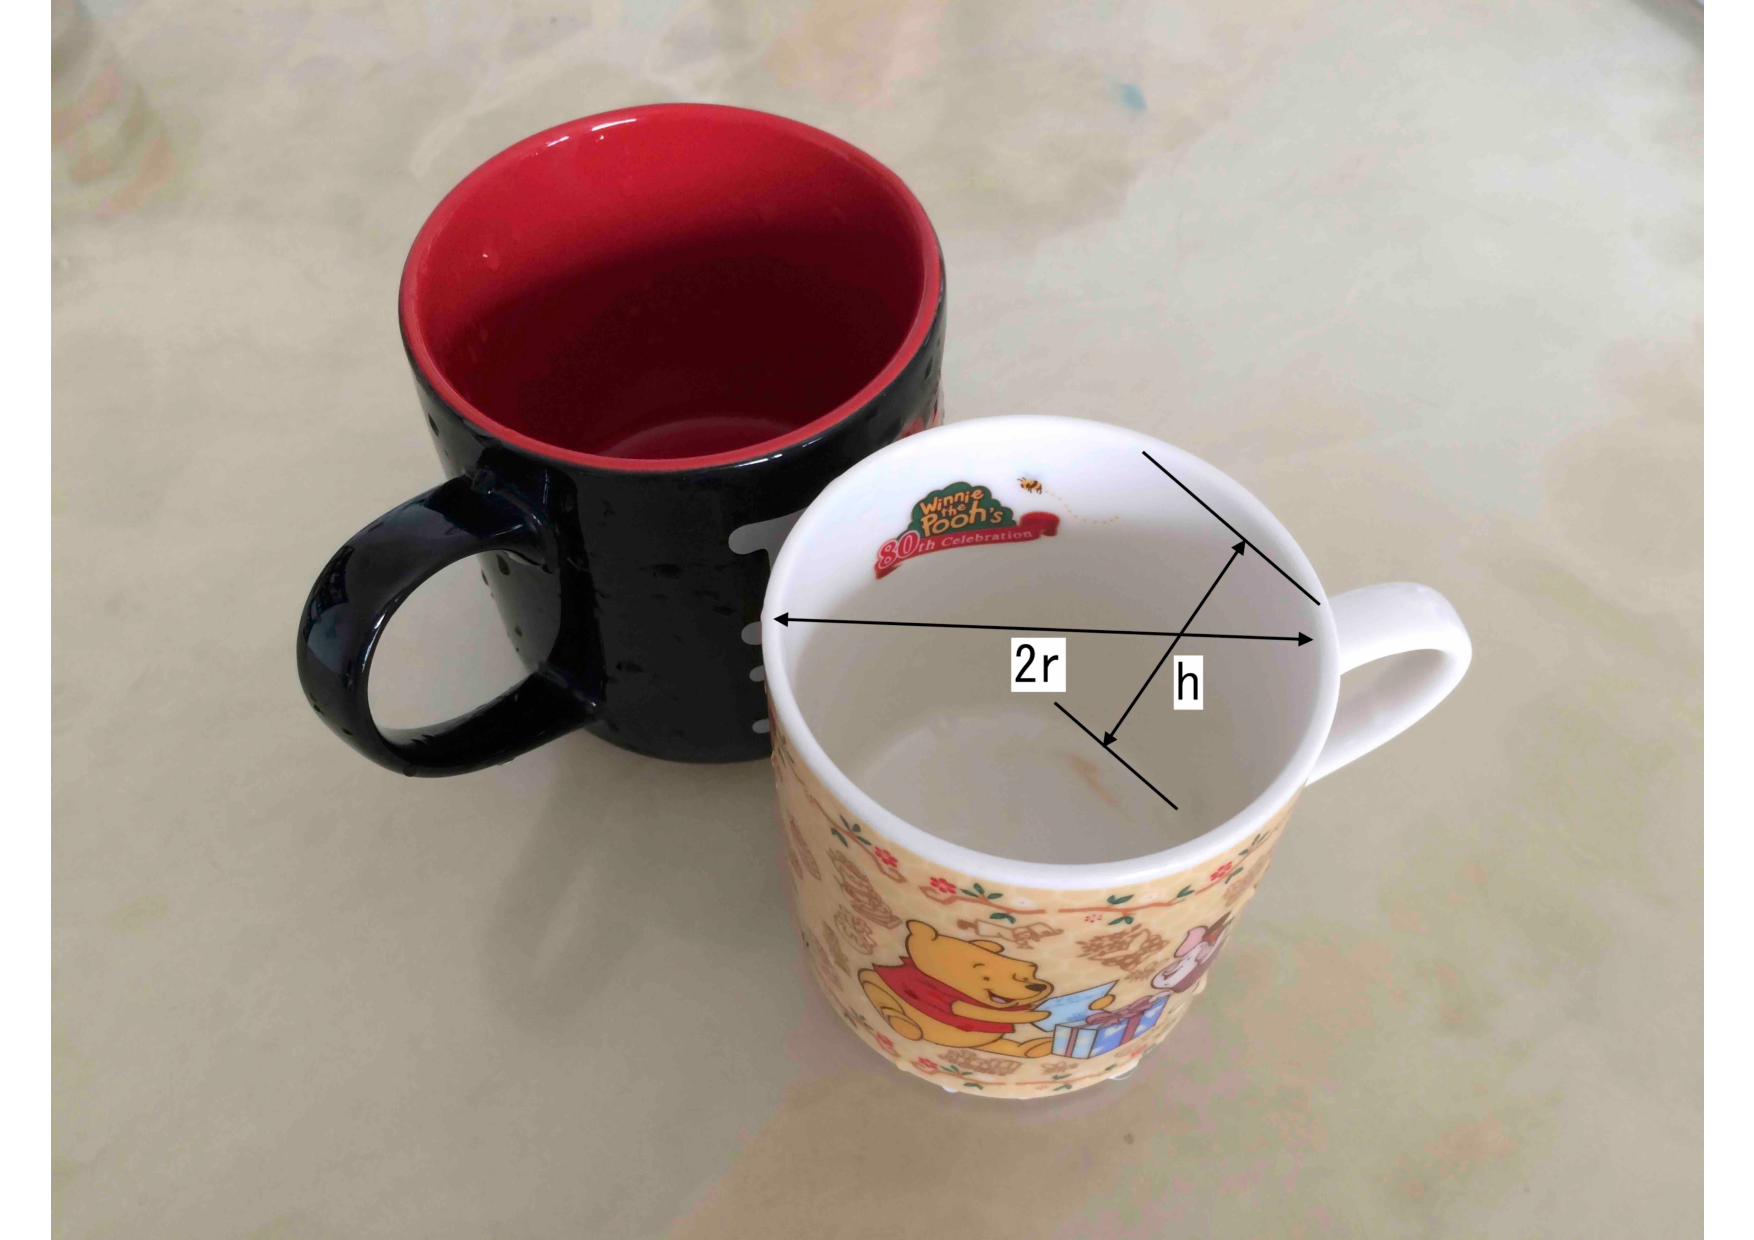
\includegraphics[keepaspectratio,scale=0.17]{cups.pdf}%
\caption{wrapfigureのテスト}
\end{wrapfigure}
湖に野生してる蓮の花がそよ風に揺れ、時折不規則的に水面に触れる。
水面から$25$センチ突き出ている蓮の花をじっと見ていたら、
$53$センチ前後離れた水面に触れることに段々と確信した。
しかし、離れる距離は目測であり、誤差が伴うことも承知する。
この誤差は、平均が$0$センチ, 標準偏差が$5$センチの正規分布に従うとしよう。
\begin{enumerate}
\item 水の深さの期待値は何センチか。
\item 水の深さが$40$センチ以上となる確率はいくらか。
\end{enumerate}
\end{問題}

確率変数の関数の分布や積率母関数の求め方を理解することが前提である。

\begin{解説}
	$X\sim N(\mu,1)$とする。$\mu =0$のとき、すなわち、$X$が標準正規分布$N(0,1)$に従うとき,$X^2$は自由度$1$のカイ自乗分布に従う。ここで、$-\infty < \mu < \infty $として、$Y=X^2$の密度関数$f(y)$と積率母関数$M(t)$を求めてみよう。

$\Phi(\cdot)$を$N(0,1)$の分布関数とする。$X-\mu \sim N(0,1)$に注意すると、任意の$y> 0$に対して、$Y$の分布関数は
\begin{eqnarray*}
F(y) &=& \mathrm{Pr}[ Y \le y] = \mathrm{Pr}[ X^2 \le y] \\
&=& \mathrm{Pr}[ -\sqrt{y} \le X \le \sqrt{y}]  \\
&=& \mathrm{Pr}[ -\sqrt{y}- \mu \le X-\mu  \le \sqrt{y}-\mu ]  \\
&=& 1 - \Phi(-\sqrt{y}- \mu) + \Phi(\sqrt{y}+ \mu)
\end{eqnarray*}
となり、$Y=X^2$の密度関数 $f(y) = F'(y)$は次のように書ける。

\begin{網掛け}
\begin{equation}
f(y) = \displaystyle
{1\over \sqrt{2\pi y}}e^{-{1\over 2}(y+\mu^2)} \cosh(\mu \sqrt{y}) \quad (y>0)
\label{eqn:pdfncc2}
\end{equation}
\end{網掛け}
ただし、
$\displaystyle \cosh x= (e^{x}+e^{-x})/2$
は双曲線余弦関数である。一方、積率母関数は次のように計算できる。
\begin{eqnarray}
M(t) &=& \mathbb E[e^{tY}] = \mathbb E[e^{tX^2}] \nonumber \\
&=& \int_{-\infty}^{\infty} e^{tx^2} {1\over \sqrt{2\pi}} 
  e^{-{1\over 2} (x-\mu)^2}\, dx \nonumber \\
&=& \displaystyle {1\over\sqrt{1-2t}} e^{{t\mu^2 \over 1-2t}}\qquad (t<1/2)
\label{eqnmgfncc}
\end{eqnarray}
$M(t)$を$t$について微分することにより、$Y$の$1$次と$2$の積率を求めることができる。
\begin{網掛け}
\begin{eqnarray}
&& \mathbb E (Y) = M'(0) = \mu^2+1 
\label{eqn:meanncc2}
\\
&& \mathbb E (Y^2) = M''(0) = \mu^4 + 6\mu^2 + 3
\end{eqnarray}
\end{網掛け}
\end{解説}

\begin{解答}
\begin{enumerate}
\item[(1)] 
蓮の花の長さは、水面に出ている部分$a=25$(cm)と、水の深さ$Y$(cm)の和からなる。条件により、蓮の花が水面に触れるときの距離を$W$(cm)とすると、
$$
W= b + \mbox{誤差} = b + N(0,\sigma^2) = N(b, \sigma^2)
$$
となる。ただし、$b=53$(cm), $\sigma=5$(cm)である。三平方の定理
$$
(Y + a)^2 = Y^2 + W^2
$$
により、$Y = W^2/(2a)$となる。$X= W/\sigma,\, \mu = b/\sigma$とすると、$X\sim N(\mu, 1)$, 
\begin{equation}
Y= {\sigma^2 \over 2 a} X^2
\label{eqn:yhasu}
\end{equation}
となる。(\ref{eqn:meanncc2})により、水の深さ$Y$の期待値は 
\begin{equation}
\mathbb E(Y) = {\sigma^2 \over 2 a} \mathbb E(X^2)  = {\sigma^2 \over 2 a} \left({b^2 \over \sigma^2} +1\right)
= {b^2 + \sigma^2 \over 2 a}
\end{equation}
となる。具体的数値を代入すると、
$\mathbb E(Y) = 56.68$(cm)となる。測定誤差がなければ、$\sigma=0$となり、$\mathbb E(Y) = b^2/(2a)$となる。これが「ハスの問題」\footnote{マーチン・ガードナー (編), 田中勇 (訳)、サム・ロイドのパズル百科, 1966 白揚社} として知られている。

\item[(2)] 
次に、$Y \ge c=40$(cm)の確率を求める。$\lambda = 2ac/\sigma^2$とすると、(\ref{eqn:yhasu}), (\ref{eqn:pdfncc2})より、
\begin{eqnarray}
\mathrm{P} [ Y\ge c] &=& \mathrm{P} [ X^2\ge \lambda] \nonumber \\
&=& \int_\lambda^\infty {1\over \sqrt{2\pi y}}e^{-{1\over 2}(y+\mu^2)} \cosh(\mu \sqrt{y})\, dy \nonumber \\
&=& \int_\lambda^\infty {1\over \sqrt{2\pi y}}e^{-{1\over 2}(y+\mu^2)} 
{e^{\mu \sqrt{y}} + e^{-\mu \sqrt{y}} \over 2} \, dy \nonumber \\
&=& 2- \Phi\left(\sqrt{\lambda} + \mu\right) -  \Phi\left(\sqrt{\lambda} - \mu\right) \nonumber \\
&=& 2- \Phi\left({\sqrt{2ac} \over \sigma}+ {b \over \sigma} \right) -  \Phi\left({\sqrt{2ac} \over \sigma} - {b \over \sigma} \right) \nonumber \\
&=& 2- \Phi\left({\sqrt{2ac} + b \over \sigma} \right) -  \Phi\left({\sqrt{2ac} - b \over \sigma} \right) \nonumber
\end{eqnarray}
ここで、$\Phi\left[{(\sqrt{2ac} + b) / \sigma} \right]\approx 1$に注意すると、
\begin{equation}
\mathrm{P} [ Y\ge c]\approx 1-  \Phi\left({\sqrt{2ac} - b \over \sigma} \right)
\end{equation}
となる。具体的数値を代入すると、
$$
\mathrm{P} [ Y\ge 40]\approx 1-  \Phi\left(-1.656 \right) \approx 0.95 = 95\%
$$
となる。

\end{enumerate}
\end{解答}
\pagebreak
\begin{teatime}[実験の計画が重要である:円周率の推定の場合]
データを要約したら、データを支配する法則を推量したりする方法論の構築が統計学の使命である。しかし、統計的方法論の選択よりも、まず質の高いデータの取得がより重要であることを肝に銘じてほしい。ここで円周率$\pi$を未知の定数として、$\pi$を推定する問題を通して実験計画の重要性を考えよう。
%\end{teatime}

\begin{wrapfigure}[11]{l}[0mm]{50mm} 
\vspace*{-\intextsep}
\centering
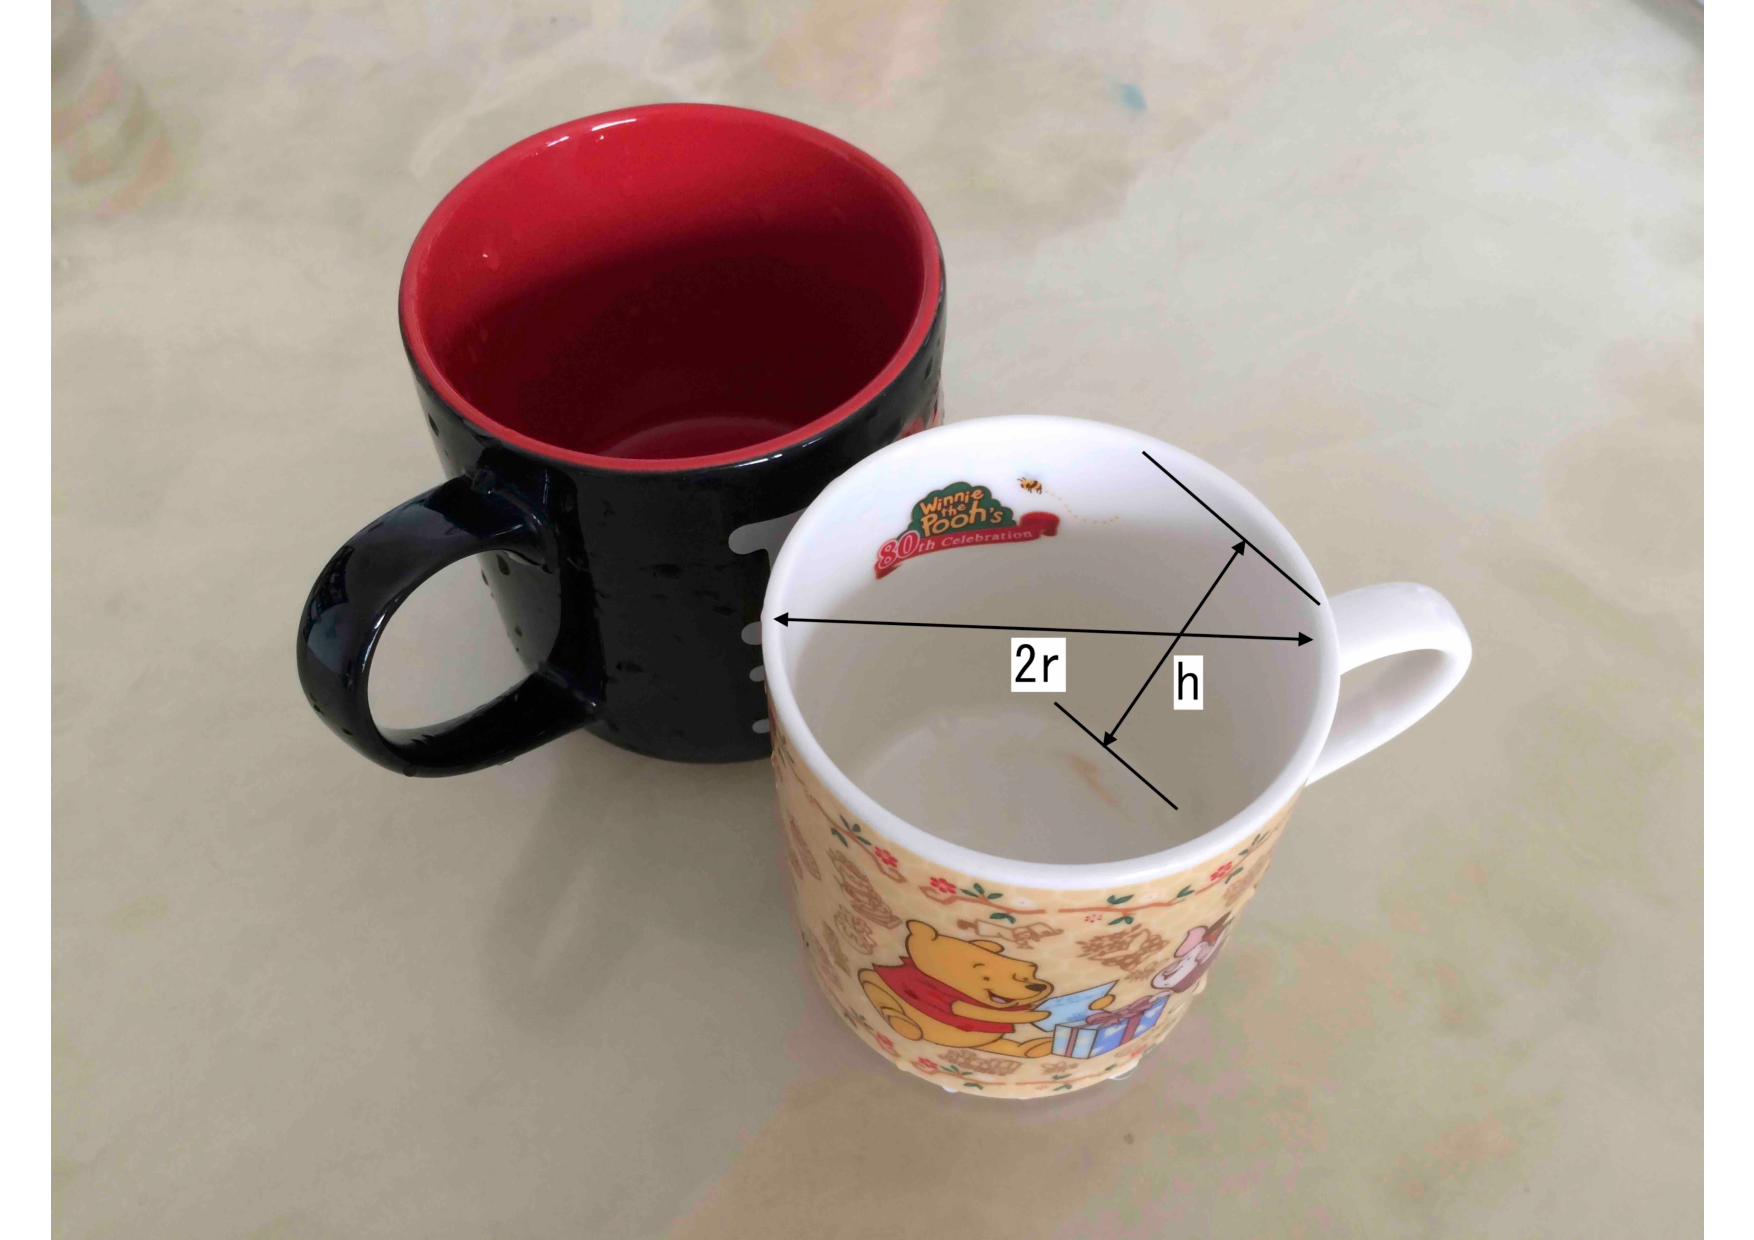
\includegraphics[keepaspectratio,scale=0.17]{cups.pdf}%
\caption{同じ高さのマグカップ\label{cup}}
\end{wrapfigure}

半径$r$、高さ$h$の円柱状のマグカップの容積は
$$
V_c = \mbox{底面積} \times \mbox{高さ} = (\pi r^2) \times h 
$$
となるので、
%半径$r$と高さ$h$の測定に誤差がないとすれば、
円周率は
\begin{equation}
\pi  = {V_c \over h r^2}
\label{eqn:pi}
\end{equation}
となる。しかし、容積$V_c$が分からないので、次のように間接的に$V_c$を
測る\footnote{このアイデアは祁華(2017, Private Communications)からヒントを得ている。}。

\begin{wrapfigure}[11]{r}[0mm]{50mm} 
\vspace*{-\intextsep}
\centering
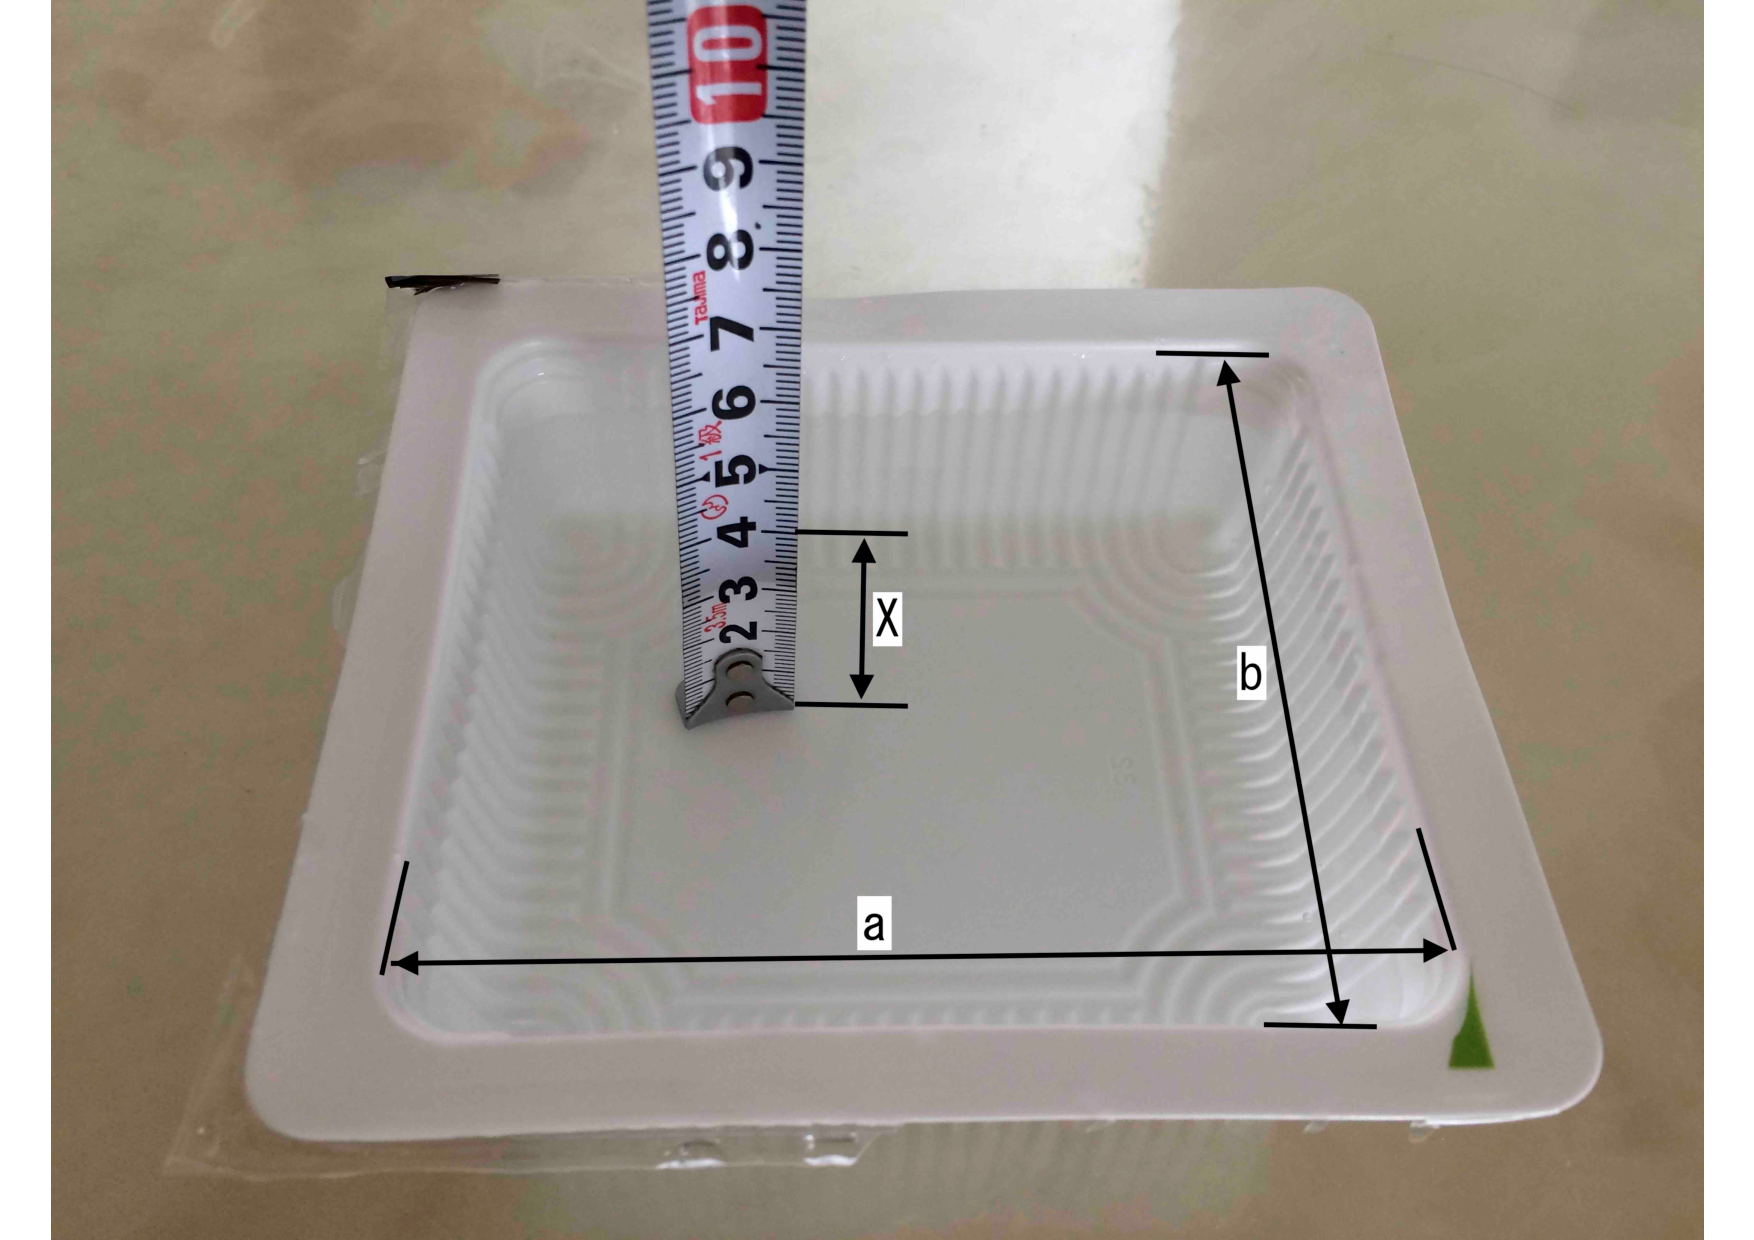
\includegraphics[keepaspectratio,scale=0.17]{toufu.pdf}%
\caption{一丁$400$g入れの豆腐容器\label{tofu}}
\end{wrapfigure}

図\ref{tofu}は、横幅$a=95$mm、縦幅$b=110$mm、一丁$400$g入れの豆腐容器である。マグカップにある満杯の水を
豆腐容器にいれ、水の深さ$X$(mm)を測る。
豆腐容器内の水の体積は
$$
V_t = a\times b\times X \qquad (\mbox{mm}^3)
$$
であり、これがマグカップの容積$V_c$の間接的な測定値と見なせる。

上の議論により、円周率の推定値として
\begin{equation}
\hat \pi = {V_t \over h r^2 } = { a b \over h r^2 }X
\end{equation}
を得る。$X$以外を定数として、$\hat\pi$の精度を表す標準偏差は
\begin{equation}
\sqrt{\mbox{V}(\hat \pi)} = \sqrt{{ a^2 b^2 \over h^2 r^4 }\mbox{V}(X)}  \propto  1/r^2
\label{eqn:pivar}
\end{equation}
となり、マグカップの半径の$2$乗に応じて減少する。従って、円周率のよい推定量を得るため、できるだけ大口のマグカップを使うべきであることが分かる。
表\ref{cuppi}は図\ref{cup}のマグカップを使った実験結果を纏めたものである。大口のカップを使った場合、一桁の精度向上が見られた。
\begin{table}[h]
\begin{center}
\begin{tabular}{c|ccc|c}
\hline \noalign{\hrule height 0.5pt}
{\bf マグカップ}  & {\bf 半径}$r$ & {\bf 深さ} $h$ & {\bf 水の深さ}$X$ & $\hat\pi = { a b \over h r^2 }X $\\
\hline \noalign{\hrule height 0.3pt}
小口カップ &  $36^{}$ &  $79$ & $31$ & ${323950 \over 102384}\approx 3.164$ \\
大口カップ &  $41_{}$ &  $79$ & $40$ & ${418000 \over 132799}\approx 3.148$ \\
\hline \noalign{\hrule height 0.5pt}
\end{tabular}
\caption{大小のマグカップによる円周率の推定値の比較\label{cuppi}}
\end{center}
\end{table}
\end{teatime}


\begin{TEST}
	\begin{SQenumerate}%% □でlabelを囲ったenumerate環境
		\item\dumyword{106}
		\item\dumyword{95s}
	\end{SQenumerate}
\end{TEST}
\begin{TEST}
	\begin{SQenumerate}
		\item\dumyword{10}
		\item\dumyword{10}
	\end{SQenumerate}
\end{TEST}


       %第1章
\include{./sampletexfiles/shuffleTEST}  %TESTshuffle20
\printindex


\end{document}

[width=]{}